\begin{figure}[htbp]
  \centering 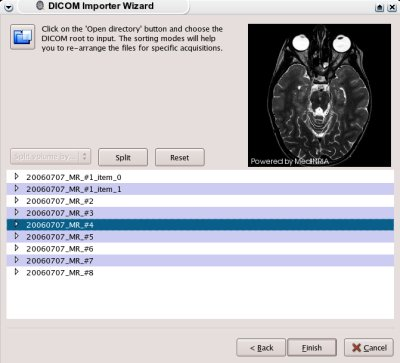
\includegraphics[width=0.65\linewidth]{dicomimport}
  \caption{{\bf The DICOM importer main window, shown with brain exam loaded. Click
      ``Open'' button to set the directory to scan.}
  \label{fig:dicomimport}}
\end{figure}

The DICOM importer is a simple wizard that allow the user to import images directly from
a DICOM exam. It can reconstruct 3D volumes from 2D DICOM files. 

IMPORTANT : This tool does not import 3D DICOM files ! You can open them directly from the
open button. 
\ \\

First click on the ``Open'' button to choose the DICOM root directory that contains the
exam. Carefull : the importer will scan recursively into this directory, don't choose a
directory that contain several exams to prevent from memory overloads.
\ \\

The volumes should now appear in the main table window. Each line with an arrow represents a
volume. Double click on it to see what files this volume is made from. Clicking on one
file will popup the corresponding image on the view window in the upper right corner. The
files should be shown in correct order, following a consistent strategy : files are first
splited in series and ordered by the image position DICOM flag. If for some reason the
user ends up with a mixed up volume, it might be because of image position conflicts (It
often happen in T2/proton density protocols). Then the user can click on ``split'' button
that provides a consistent split process among the image positions given in the DICOM
files. Clicking on reset button will go back to the original configuration.

Last step (click ``finish'') will reconstruct 3D volumes from the last given fileset
configuration.
\ \\

IMPORTANT : The DICOM importer in its current state doesn't take care of the orientation
acquisiton of the the image. That might results in ``radiologic convention'' issues.
\ \\

